\section{Day 2: Course Overview (Sep. 4, 2024)}
To start, recall that a binary quadratic form is given by $f(x, y) = ax^2 + bxy + cy^2$, where $a, b, c$ are in some number field, preferably working in $\ZZ$. We say that $f(x, y) \sim g(x, y)$ if there exists $\gamma \in \SL_2(\ZZ)$ such that $g(x, y) = f((x, y) \gamma^T)$ (notational convention).

\subsection{Week 2}
\begin{simplethm}[Gauss]
    Equivalence classes of binary quadratic forms of a fixed discriminant $D$ form a finite abelian group.
\end{simplethm}
\noindent Specifically, $\mathrm{disc}(f(x, y)) = b^2 - 4ac$. The narrow class group is a variant of the class group $\mathrm{Cl}(\QQ(\sqrt{D}))$, of which the latter should be interpreted as the class group of quadratic field $\QQ(\sqrt{D})$. This is equal to the fractional ideals of $\QQ(\sqrt D)$ modulo the principal ideals of $\QQ(\sqrt D)$. If $\mathrm{Cl}(\QQ(\sqrt{D}))$ is trivial, then there is unique factorization; otherwise, it has unique factorization of ideals into prime ideals.

\begin{simplethm}
    This aforementioned finite abelian group is isomorphic to the narrow class group of $\QQ(\sqrt D)$, where $D$ is the discriminant.
\end{simplethm}

\subsection{Week 3}
This week will introduce the Bhargava cube, where
\begin{center} 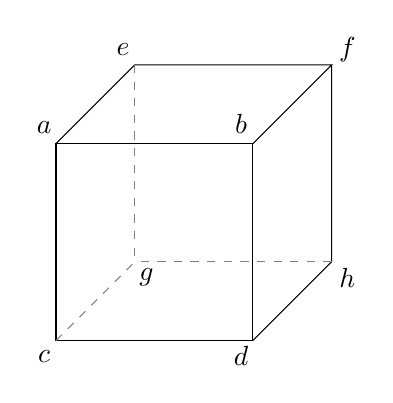
\begin{tikzpicture}[scale=0.5]
    \draw (0, 0) -- (5, 0) -- (5, 5) -- (0, 5) -- cycle;
    \draw (0, 5) -- (2, 7) -- (7, 7) -- (5, 5);
    \draw (5, 0) -- (7, 2) -- (7, 7);
    \draw[dashed, gray] (0, 0) -- (2, 2);
    \draw[dashed, gray] (7, 2) -- (2, 2);
    \draw[dashed, gray] (2, 7) -- (2, 2);
    \node at (-0.3, -0.4) {$c$};
    \node at (-0.3, 5.4) {$a$};
    \node at (4.7, 5.5) {$b$};
    \node at (4.7, -0.4) {$d$};
    \node at (1.7, 7.4) {$e$};
    \node at (7.4, 7.4) {$f$};
    \node at (7.4, 1.6) {$h$};
    \node at (2.3, 1.6) {$g$};
\end{tikzpicture} \end{center}
Taking pairs of opposite faces, we obtain $3$ pairs of $2 \times 2$ matrices that we may use to obtain $3$ binary quadratic forms, such as
\[ Q_1(x, y) := \det \begin{pmatrix} ax - ey & bx - fy \\ cx - gy & dx - hy \end{pmatrix}, \]
with similar definitions for $Q_2(x, y)$ and $Q_3(x, y)$; we may note that $Q_1, Q_2, Q_3$ have the same discriminant. These induce a cube law where $[Q_1] \cdot [Q_2] \cdot [Q_3]$ is the identity equivalence class. This reinterprets Gauss' composition law. In particular, we may construct a bijection between the equivalence classes of cubes with discrminant $D$, and the ideal classes $(I_1, I_2, I_3)$ with $I_1 \cdot I_2 \cdot I_3 \subseteq S_p$.

\newpage
\subsection{Week 4}
We construct a symmetric Bhargava cube, where all six of the matrices obtained are symmetric; such a construction follows,
\begin{center} 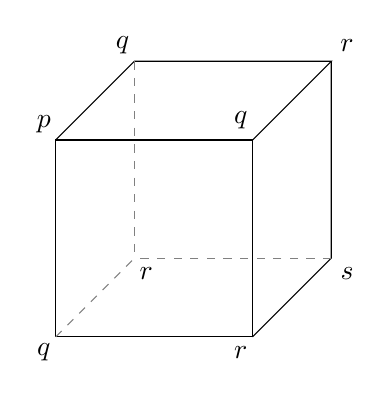
\begin{tikzpicture}[scale=0.5]
    \draw (0, 0) -- (5, 0) -- (5, 5) -- (0, 5) -- cycle;
    \draw (0, 5) -- (2, 7) -- (7, 7) -- (5, 5);
    \draw (5, 0) -- (7, 2) -- (7, 7);
    \draw[dashed, gray] (0, 0) -- (2, 2);
    \draw[dashed, gray] (7, 2) -- (2, 2);
    \draw[dashed, gray] (2, 7) -- (2, 2);
    \node at (-0.3, -0.4) {$q$};
    \node at (-0.3, 5.4) {$p$};
    \node at (4.7, 5.5) {$q$};
    \node at (4.7, -0.4) {$r$};
    \node at (1.7, 7.4) {$q$};
    \node at (7.4, 7.4) {$r$};
    \node at (7.4, 1.6) {$s$};
    \node at (2.3, 1.6) {$r$};
\end{tikzpicture} \end{center}
This yields a binary cubic form $px^3 + 3qx^2y + 3rxy^2 + sy^3$, and it induces a bijection from the $\SL_2(\ZZ)$ equivaelnce class of binary cubic forms of discriminant $D$ to the $3$-torsion ideal class elements of quadratic rings $S_p = \ZZ[\frac{D + \sqrt{D}}{2}]$. The discriminant formula may be obtained with Viete's formulas and by taking the product over the difference of roots pairwise.

\subsection{Week 5 - Higher Composition Laws}
\begin{simplethm}[Levi, Delone-Fadeev, Gan-Gross-Savin]
    Let us have binary cubic forms $f(x, y) = ax^3 + bx^2y + cxy^2 + dy^3$ over $\ZZ$; then $\gamma \in \GL_2(\ZZ)$ acts on $f$ by $\gamma f(x, y) = \frac{f((x, y) \gamma)}{\det \gamma}$.
\end{simplethm}
\noindent This induces a bijection between $\GL_2(\ZZ)$ orbits of binary cubic forms of a given discriminant $D$ with cubic rings (rank $3$ as a $\ZZ$-module) up to ring isomorphism.

\begin{simplethm}[Davenport-Heilbronn]
    There is something that bijects to maximal cubic rings at $p$. (will be expanded in class later on)
\end{simplethm}
\noindent A cubic ring is maximal if and only if it is maximal at all primes $p$; it is maximal at $p$ if and onyl if $R \otimes \ZZ_p$ is maximal.

\subsection{Week 6}
This week we will introduce $3$ new parameterizations and composition laws.
\begin{enumerate}
    \item $2 \times 3 \times 3$ boxes, which induce a bijection between pairs of $3 \times 3$ matrices and pairs of ideal class elements $I_1, I_2$ such that $I_1, I_2 \subseteq R$; i.e., $N(I_1) \cdot N(I_2) = 1$.
    \item Symmetrized $2 \times 3 \times 3$ boxes, which induce a bijection between pairs of $3 \times 3$ symmetric matrices and order $2$ ideal class elements.
    \item Bijection between binary $n$-ic forms and certain rings of rank $n$.
\end{enumerate}
Specifically, quadratic rings are parametrized by the discriminant, cubic rings by binary cubic forms, and quartic rings by pairs of $3 \times 3$ symmetric matrices, with extra structure in resolvent rings.

\noindent If $Q$ is a quartic ring, it is a rank $4$ $\ZZ$-module,
\[ Q = \left< 1, \alpha_1, \alpha_2, \alpha_3 \right> \]
with basis as a $\ZZ$-module.
\begin{simplethm}
    To every quartic ring $Q$, there is a resolvent cubic ring $R = \left< 1, \beta_1, \beta_2 \right>$ and a map $Q / \ZZ = \left< \alpha_1, \alpha_2, \alpha_3 \right> \to R / \ZZ = \left< \beta_1, \beta_2 \right>$.
\end{simplethm}

\subsection{Week 7}
\begin{simplethm}[Bhargava]
    There is a bijection between $\GL_2(\ZZ) \times \SL_3(\ZZ)$ equivalence classes of ternary quadratic forms and $(Q, R)$ (quartic rings and cubic resolvents).
\end{simplethm}

\subsection{Week 8 and Onwards}
We will look at which quartic rings are parametrized by binary quartic forms (Wood), and introduce the Davenport-Heilbronn theorem properly (?); the number of cubic fields ordered by discriminant is given by
\[ \frac{1}{3 \zeta(3)} x + o(x). \]
Then we will talk about Prof. Ila's research.